\documentclass[titlepage]{article}
\usepackage{amsmath}
\usepackage{enumitem}
\usepackage{graphicx}

\title{CS 440 - Homework 5}
\author{Matthew Liu}
\date{}

\begin{document}
\maketitle{}

\section*{Problem 1}

\noindent \textbf{1. } Is this network a polytree? If so, how do you know? If not, why not?\\

Yes, because if you replace the directed edges with undirected edges, the resulting graph is both connected and acylic.\\

\noindent \textbf{2. } How many parameters are necessary to fully express the joint distribution? How many parameters are necessary in the Bayesian network?\\

\begin{itemize}
	\item Joint Distribution: $2^n-1=2^5-1=31$ parameters
	\item Bayesian Network: $P(L)+P(U)+P(R|L)+P(G|R)+P(T|U,R)=1+1+2+2+4=10$ parameters
\end{itemize}

\noindent \textbf{3. } You checked Google Maps and there is traffic. Would finding out if it is also raining affect your belief about whether a UFO has landed on the highway? Justify your answer using conditional independence rules.\\

Yes it would decrease my belief of the UFO landing on the highway. Per the Bayesian Net, $P(T)$ is conditionally dependent on $P(U)$ and $P(R)$. Whether or not it rains does not directly influence whether there is a ufo (as there is no connection between them in the net, hence they are independent). However, both of them influence traffic, and if it is raining, I am more likely to assume that rain is the reason for the traffic. If I do not know whether it is raining, I would follow conditional probabilities. Hence $P(U), P(R)$ are not conditionally independent.\\

\noindent \textbf{4. } You check your barometer and you see that there is a low pressure outside. Does this give you any information about whether a UFO landed on the highway? Justify your answer using conditional independence rules.\\

Yes. $L$ influences $R$, $(P(R|L))$ in the Bayesian Net, and $R$ influences $T$, $P(T|U,R)$. The rest of the argument follows 3 (above).\\

\noindent \textbf{5. } Does knowing there is a low pressure give you any information about whether there is traffic? Justify your answer using conditional independence rules.\\

Yes. $L$ influences $R$, $(P(R|L))$ in the Bayesian Net, and $R$ influences $T$, $P(T|U,R)$. Hence, knowing there is low pressure means it is more likely to have rain, and thus more likely to have traffic.\\

\noindent \textbf{6. } Assume that we observe the data on the right, and we want to estimate the parameters of this network:
\begin{itemize}
	\item Compute the most likely distribution \textit{P(U)} with no smoothing
	\begin{itemize}
		\item $P(U) = \frac{0}{6} = 0$
		\item $P(\neg U) = \frac{6}{6} = 1$
	\end{itemize}
	\item Compute \textit{P(U)} with Laplace smoothing with a smoothing constant 1
	\begin{itemize}
		\item $P(U) = \frac{0+1}{6+1+1} = 0.125$
		\item $P(\neg U) = \frac{6+1}{6+1+1} = 0.875$
	\end{itemize}
	\item Which of these would you expect to be a better model of the real world? Explain.\\
		I would expect the distribution with laplace smoothing to be a better model. We can not say for certain that there are no aliens, and thus can not conclusively state that it is impossible for a UFO to land on the highway (as the distributio with no smoothing states $P(U)=0$).
\end{itemize}

\noindent \textbf{7. } For the next parts, use the following as the parameters of the network\\

\centerline{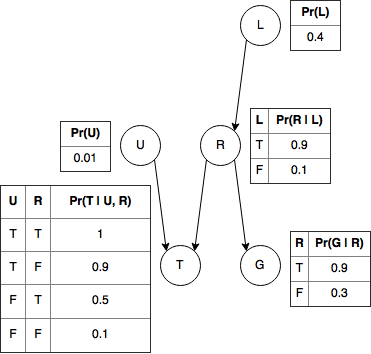
\includegraphics[scale=0.7]{7params.png}}
\begin{enumerate}[label=(\alph*)]
	\item Compute $P(G=1)$\\
		\begin{equation*}
		\begin{aligned}
			P(G=1) &= P(R)*0.9+P(\neg R)*0.3\\
				   &= [P(L) * 0.9 + P(\neg L) * 0.1] * 0.9 + [P(L) * 0.1 + P(\neg L) * 0.9] * 0.3\\
				   &= [0.4 * 0.9 + 0.6 * 0.1] * 0.9 + [0.4 * 0.1 + 0.6 * 0.9] * 0.3\\
				   &= 0.552
		\end{aligned}
		\end{equation*}
	\item Compute $P(G=1|L=0)$\\
		\begin{equation*}
		\begin{aligned}
			P(G=1|L=0) &= P(G | \neg L)\\
					   &= P(R|\neg L)*0.9+P(\neg R|\neg L)*0.3\\
					   &= 0.1 * 0.9 + 0.9 * 0.3\\
					   &= 0.36
		\end{aligned}
		\end{equation*}
	\item Computer the joint probability $P(L=1,R=1,G=0,T=0,U=0)$\\
	\begin{equation*}
	\begin{aligned}
		P(\text{L=1, R=1, G=0, T=0, U=0}) &= P(L, R, \neg G, \neg T, \neg U)\\
										  &= P(L) * P(R|L) * P(\neg G | R,L) * P(\neg T | R, \neg U) * P(\neg U)\\
		 								  &= 0.4 * [0.4 * 0.9] * [P(R|L) * 0.1] * [P(R|L) * P(\neg U) * 0.5] * 0.99\\
		 								  &= 0.4 * 0.36 * [(0.4 * 0.9) * 0.1] * [(0.4 * 0.9) * (0.99) * 0.5] * 0.99\\
		 								  &= 0.4 * 0.36 * [(0.4 * 0.9) * 0.1] * [(0.4 * 0.9) * (0.99) * 0.5] * 0.99\\
		 								  &= 0.000915
	\end{aligned}
	\end{equation*}
\end{enumerate}

\noindent \textbf{8. } Specify the Markov blanket for each random variable in this Bayesian network.\\
\begin{itemize}
	\item $MB(L)$: \{R\}
	\item $MB(R)$: \{L, G, U, T\}
	\item $MB(G)$: \{R\}
	\item $MB(U)$: \{R, T\}
	\item $MB(T)$: \{U, R\}
\end{itemize}


\pagebreak

\section*{Problem 2}

\noindent \textbf{1. } How many parameters are required to represent a full joint distribution?\\

$3 * 2 * 2 * 3 - 1 = 2^2 * 3^2 - 1= 35$ parameters\\

\noindent \textbf{2. } Give the ordering: GAS, START, HORN, BATT, draw the Bayesian network. You may optionally explain any non-intuitive decisions.\\

\centerline{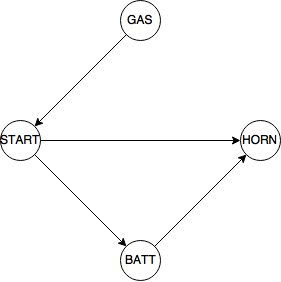
\includegraphics[scale=0.5]{22.png}}

\noindent \textbf{3. } How many parameters are required to represent the distribution using your Bayesian network of part 2?\\

\begin{equation*}
\begin{aligned}
\text{Parameters} &= P(\text{GAS})+P(\text{START$|$GAS})+P(\text{BATT$|$START})+P(\text{HORN$|$START,BATT})\\
				  &= 2+3+3+6\\
				  &= 14
\end{aligned}
\end{equation*}

\pagebreak

\noindent \textbf{4. } What is the best Bayesian network ordering you can think of for these random variables?\\

BATT, HORN, START, GAS\\

\noindent \textbf{5. } Draw another Bayesian network using the ordering you came up with in part 4. You may optionally explain any non-intuitive decisions.\\

\centerline{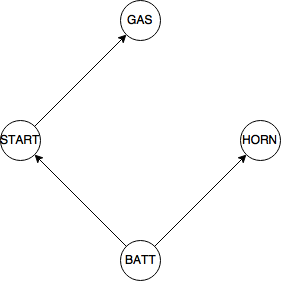
\includegraphics[scale=0.5]{25.png}}

\noindent \textbf{6. } How many parameters are required to represent the distribution using your network of part 5?\\
\begin{equation*}
\begin{aligned}
\text{Parameters} &= P(\text{BATT})+P(\text{HORN$|$BATT})+P(\text{START$|$BATT})+P(\text{GAS$|$START})\\
				  &= 2+3+3+3\\
				  &= 11
\end{aligned}
\end{equation*}

\end{document}